\documentclass[10pt,a4paper]{article}
\usepackage[utf8]{inputenc}
\usepackage[top=2cm,bottom=2cm,left=2cm,right=2cm]{geometry}
\usepackage{amsmath}
\usepackage{amssymb}
\usepackage{array}
\usepackage{tikz}
\usetikzlibrary{arrows.meta,calc,patterns,positioning}
\usepackage{pgfplots}
\pgfplotsset{compat=1.18}
\usepackage[dvipsnames,svgnames]{xcolor}
\usepackage{hyperref}

% Anchor persamaan unik meski nomor di-reset per soal.
\newcounter{eqblock}
\newcommand{\reseteq}{%
  \stepcounter{eqblock}%
  \setcounter{equation}{0}%
  \renewcommand{\theHequation}{\arabic{eqblock}.\arabic{equation}}%
}

\pgfplotsset{
  grafik/.style={
    axis lines=middle,
    xlabel={$x$}, ylabel={$y$},
    width=7.5cm, height=6cm,
    grid=major, grid style={gray!25},
    tick label style={font=\scriptsize},
    every axis x label/.style={at={(ticklabel* cs:1)},anchor=west},
    every axis y label/.style={at={(ticklabel* cs:1)},anchor=south},
    title style={yshift=2ex},
  },
}

\title{Tugas Minggu 5 : Kekontinuan}
\author{Matematika untuk Sistem Informasi}
\date{}

\begin{document}

\maketitle

\begin{enumerate}

%===========================================================
\item Diketahui
\[
f(x) =
\begin{cases}
  x^2 - 1, & x \leq -1 \\
  2x + 2, & x > -1
\end{cases}
\]
selidiki kekontinuan fungsi $f$ di $x = -1$.

\textbf{Jawab:}
\begin{itemize}
\item \textbf{Langkah 1: Hitung $f(-1)$}

\reseteq
\begin{align}
f(-1) &= (-1)^2 - 1 = 1 - 1 = 0 \quad \text{(Aturan untuk $x \leq -1$)}
\end{align}
Syarat ke-1 terpenuhi: $f(-1)$ terdefinisi.

\item \textbf{Langkah 2: Hitung Limit Kiri dan Limit Kanan}

Aturan fungsi berubah di $x = -1$, sehingga limit dihitung dari kedua arah.
\reseteq
\begin{align}
\lim_{x \to -1^-} f(x) &= \lim_{x \to -1^-} (x^2 - 1) = (-1)^2 - 1 = 0 \quad \text{(Aturan untuk $x < -1$)} \\
\lim_{x \to -1^+} f(x) &= \lim_{x \to -1^+} (2x + 2) = 2(-1) + 2 = 0 \quad \text{(Aturan untuk $x > -1$)}
\end{align}
Limit kiri sama dengan limit kanan, sehingga $\lim_{x \to -1} f(x) = 0$ ada (syarat ke-2 terpenuhi).

\item \textbf{Langkah 3: Bandingkan Limit dengan Nilai Fungsi}

Karena $\lim_{x \to -1} f(x) = 0 = f(-1)$, syarat ke-3 terpenuhi.
Jadi $f$ \textbf{kontinu} di $x = -1$.
% final: \text{kontinu di } x = -1
\end{itemize}

%===========================================================
\item Diberikan fungsi berikut:
\[
f(x) =
\begin{cases}
  2x, & x \leq -1 \\
  x^2 - 1, & -1 < x < 2 \\
  4 - x, & x \geq 2
\end{cases}
\]
\begin{enumerate}

%-----------------------------------------------------------
\item Gambarkan grafik fungsi tersebut.

\textbf{Jawab:}
\begin{itemize}
\item \textbf{Langkah 1: Hitung Nilai di Ujung Setiap Potongan}

\begin{center}
\begin{tabular}{c|c|c|c}
Potongan & Selang & Ujung kiri & Ujung kanan \\ \hline
$2x$ & $x \leq -1$ & $x \to -\infty$ & $(-1,-2)$ penuh \\
$x^2 - 1$ & $-1 < x < 2$ & $(-1,0)$ kosong & $(2,3)$ kosong \\
$4 - x$ & $x \geq 2$ & $(2,2)$ penuh & $x \to \infty$
\end{tabular}
\end{center}
Titik bantu lain: $f(-2) = -4$, $f(0) = -1$ (puncak terendah parabola), $f(1) = 0$, dan $f(3) = 1$.

\item \textbf{Langkah 2: Gambar Grafik}

\begin{center}
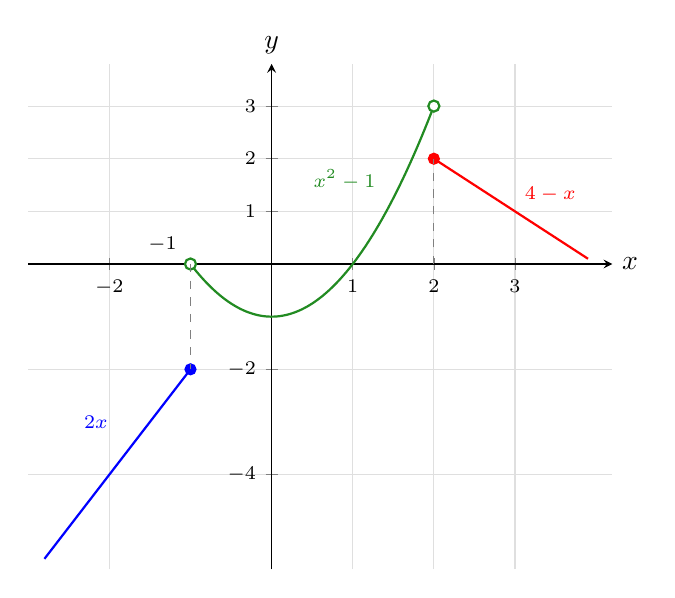
\begin{tikzpicture}
\begin{axis}[grafik, width=9cm, height=8cm, xmin=-3, xmax=4.2, ymin=-5.8, ymax=3.8,
  xtick={-2,1,2,3}, ytick={-4,-2,1,2,3}]
  \addplot[domain=-2.8:-1, thick, blue] {2*x};
  \addplot[domain=-1:2, samples=80, thick, ForestGreen] {x^2 - 1};
  \addplot[domain=2:3.9, thick, Red] {4 - x};
  \filldraw[blue] (axis cs:-1,-2) circle (2pt);
  \filldraw[ForestGreen, fill=white, thick] (axis cs:-1,0) circle (2pt);
  \filldraw[ForestGreen, fill=white, thick] (axis cs:2,3) circle (2pt);
  \filldraw[Red] (axis cs:2,2) circle (2pt);
  \draw[dashed, gray] (axis cs:-1,0) -- (axis cs:-1,-2);
  \node[font=\scriptsize, anchor=south east] at (axis cs:-1.05,0.05) {$-1$};
  \draw[dashed, gray] (axis cs:2,0) -- (axis cs:2,2);
  \node[font=\scriptsize, blue, anchor=east] at (axis cs:-1.9,-3) {$2x$};
  \node[font=\scriptsize, ForestGreen, anchor=east] at (axis cs:1.4,1.6) {$x^2 - 1$};
  \node[font=\scriptsize, Red, anchor=south west] at (axis cs:3,1) {$4 - x$};
\end{axis}
\end{tikzpicture}
\end{center}
Grafik terputus (melompat) di $x = -1$ dan di $x = 2$.
\end{itemize}

%-----------------------------------------------------------
\item Periksa apakah fungsi tersebut kontinu di titik $x = -1$ dan $x = 2$.

\textbf{Jawab:}
\begin{itemize}
\item \textbf{Langkah 1: Kekontinuan di $x = -1$}

\reseteq
\begin{align}
f(-1) &= 2(-1) = -2 \quad \text{(Aturan untuk $x \leq -1$)} \\
\lim_{x \to -1^-} f(x) &= \lim_{x \to -1^-} 2x = -2 \quad \text{(Aturan untuk $x < -1$)} \\
\lim_{x \to -1^+} f(x) &= \lim_{x \to -1^+} (x^2 - 1) = (-1)^2 - 1 = 0 \quad \text{(Aturan untuk $-1 < x < 2$)}
\end{align}
Karena $\lim_{x \to -1^-} f(x) = -2 \neq 0 = \lim_{x \to -1^+} f(x)$, maka $\lim_{x \to -1} f(x)$ tidak ada (syarat ke-2 tidak terpenuhi).
Jadi $f$ \textbf{tidak kontinu} di $x = -1$ (diskontinuitas lompat).
Namun $\lim_{x \to -1^-} f(x) = -2 = f(-1)$, sehingga $f$ \textbf{kontinu kiri} di $x = -1$.

\item \textbf{Langkah 2: Kekontinuan di $x = 2$}

\reseteq
\begin{align}
f(2) &= 4 - 2 = 2 \quad \text{(Aturan untuk $x \geq 2$)} \\
\lim_{x \to 2^-} f(x) &= \lim_{x \to 2^-} (x^2 - 1) = 2^2 - 1 = 3 \quad \text{(Aturan untuk $-1 < x < 2$)} \\
\lim_{x \to 2^+} f(x) &= \lim_{x \to 2^+} (4 - x) = 4 - 2 = 2 \quad \text{(Aturan untuk $x > 2$)}
\end{align}
Karena $\lim_{x \to 2^-} f(x) = 3 \neq 2 = \lim_{x \to 2^+} f(x)$, maka $\lim_{x \to 2} f(x)$ tidak ada.
Jadi $f$ \textbf{tidak kontinu} di $x = 2$ (diskontinuitas lompat).
Namun $\lim_{x \to 2^+} f(x) = 2 = f(2)$, sehingga $f$ \textbf{kontinu kanan} di $x = 2$.
% final: \text{tidak kontinu di } x = -1
% final: \text{tidak kontinu di } x = 2
\end{itemize}

\end{enumerate}

%===========================================================
\item Tentukan konstanta $a$ dan $b$ agar fungsi
\[
f(x) =
\begin{cases}
  \dfrac{x^2 - 4}{x - 2}, & x < 2 \\[1.5ex]
  ax^2 - bx + 3, & 2 \leq x < 3 \\
  2x - a + b, & x \geq 3
\end{cases}
\]
kontinu di $\mathbb{R}$.

\textbf{Jawab:}
\begin{itemize}
\item \textbf{Langkah 1: Sederhanakan dan Tentukan Titik yang Perlu Diperiksa}

Pada selang $x < 2$ berlaku $x \neq 2$, sehingga
\reseteq
\begin{align}
\frac{x^2 - 4}{x - 2} &= \frac{(x - 2)(x + 2)}{x - 2} = x + 2 \quad \text{(Coret $x - 2$, sah karena $x \neq 2$)}
\end{align}
Ketiga potongan ($x + 2$, $ax^2 - bx + 3$, dan $2x - a + b$) adalah polinom, sehingga kontinu di dalam selangnya masing-masing.
Yang perlu diperiksa hanya titik perubahan aturan, yaitu $x = 2$ dan $x = 3$.

\item \textbf{Langkah 2: Syarat Kontinu di $x = 2$}

\reseteq
\begin{align}
f(2) &= a(2)^2 - b(2) + 3 = 4a - 2b + 3 \quad \text{(Aturan untuk $2 \leq x < 3$)} \\
\lim_{x \to 2^-} f(x) &= \lim_{x \to 2^-} (x + 2) = 4 \quad \text{(Aturan untuk $x < 2$)} \\
\lim_{x \to 2^+} f(x) &= \lim_{x \to 2^+} (ax^2 - bx + 3) = 4a - 2b + 3
\end{align}
Agar kontinu, limit kiri harus sama dengan $f(2)$:
\reseteq
\begin{align}
4a - 2b + 3 &= 4 \\
4a - 2b &= 1 \quad \text{(Persamaan (i))}
\end{align}

\item \textbf{Langkah 3: Syarat Kontinu di $x = 3$}

\reseteq
\begin{align}
f(3) &= 2(3) - a + b = 6 - a + b \quad \text{(Aturan untuk $x \geq 3$)} \\
\lim_{x \to 3^-} f(x) &= \lim_{x \to 3^-} (ax^2 - bx + 3) = 9a - 3b + 3 \quad \text{(Aturan untuk $2 \leq x < 3$)} \\
\lim_{x \to 3^+} f(x) &= \lim_{x \to 3^+} (2x - a + b) = 6 - a + b
\end{align}
Agar kontinu, limit kiri harus sama dengan $f(3)$:
\reseteq
\begin{align}
9a - 3b + 3 &= 6 - a + b \\
10a - 4b &= 3 \quad \text{(Persamaan (ii))}
\end{align}

\item \textbf{Langkah 4: Selesaikan Sistem Persamaan}

\reseteq
\begin{align}
8a - 4b &= 2 \quad \text{(Kalikan (i) dengan 2)} \\
(10a - 4b) - (8a - 4b) &= 3 - 2 \quad \text{(Kurangkan dari (ii))} \\
2a &= 1 \;\Rightarrow\; a = \frac{1}{2} \\
4\left(\tfrac{1}{2}\right) - 2b &= 1 \;\Rightarrow\; 2 - 2b = 1 \;\Rightarrow\; b = \frac{1}{2} \quad \text{(Substitusi ke (i))}
\end{align}
Jadi $a = \frac{1}{2}$ dan $b = \frac{1}{2}$.
% final: a = \frac{1}{2}
% final: b = \frac{1}{2}

\item \textbf{Langkah 5: Verifikasi}

Dengan $a = b = \frac{1}{2}$, fungsi menjadi
\[
f(x) =
\begin{cases}
  x + 2, & x < 2 \\
  \frac{1}{2}x^2 - \frac{1}{2}x + 3, & 2 \leq x < 3 \\
  2x, & x \geq 3
\end{cases}
\]
\reseteq
\begin{align}
x = 2&: \quad \lim_{x \to 2^-} (x + 2) = 4, \quad f(2) = 2 - 1 + 3 = 4 \\
x = 3&: \quad \lim_{x \to 3^-} \left(\tfrac{1}{2}x^2 - \tfrac{1}{2}x + 3\right) = \tfrac{9}{2} - \tfrac{3}{2} + 3 = 6, \quad f(3) = 2(3) = 6
\end{align}
Kedua titik sambungan cocok, sehingga $f$ kontinu di $\mathbb{R}$.
\end{itemize}

%===========================================================
\item Diberikan fungsi berikut:
\[
f(x) =
\begin{cases}
  x + 3, & x \leq -1 \\
  -x + c, & -1 < x < 1 \\
  x^2 - 2x + 1, & x \geq 1
\end{cases}
\]
\begin{enumerate}

%-----------------------------------------------------------
\item Tentukan nilai $c$ agar $f(x)$ kontinu di $x = -1$.

\textbf{Jawab:}
\begin{itemize}
\item \textbf{Langkah 1: Hitung $f(-1)$ dan Limit Sepihak}

\reseteq
\begin{align}
f(-1) &= -1 + 3 = 2 \quad \text{(Aturan untuk $x \leq -1$)} \\
\lim_{x \to -1^-} f(x) &= \lim_{x \to -1^-} (x + 3) = 2 \quad \text{(Aturan untuk $x < -1$)} \\
\lim_{x \to -1^+} f(x) &= \lim_{x \to -1^+} (-x + c) = 1 + c \quad \text{(Aturan untuk $-1 < x < 1$)}
\end{align}
Fungsi sudah kontinu kiri di $x = -1$ untuk sebarang $c$; yang perlu dipenuhi adalah kontinu kanan.

\item \textbf{Langkah 2: Samakan Limit Kanan dengan $f(-1)$}

\reseteq
\begin{align}
1 + c &= 2 \quad \text{(Limit kanan $=$ $f(-1)$)} \\
c &= 1
\end{align}
Dengan $c = 1$: $\lim_{x \to -1} f(x) = 2 = f(-1)$, sehingga $f$ kontinu di $x = -1$.
% final: c = 1
\end{itemize}

%-----------------------------------------------------------
\item Berdasarkan nilai $c$ yang telah diperoleh pada bagian (a), periksa apakah $f(x)$ kontinu di $x = 1$.

\textbf{Jawab:}
\begin{itemize}
\item \textbf{Langkah 1: Hitung $f(1)$}

\reseteq
\begin{align}
f(1) &= 1^2 - 2(1) + 1 = 0 \quad \text{(Aturan untuk $x \geq 1$)}
\end{align}

\item \textbf{Langkah 2: Hitung Limit Kiri dan Limit Kanan}

Dengan $c = 1$, potongan tengahnya adalah $-x + 1$.
\reseteq
\begin{align}
\lim_{x \to 1^-} f(x) &= \lim_{x \to 1^-} (-x + 1) = -1 + 1 = 0 \quad \text{(Aturan untuk $-1 < x < 1$)} \\
\lim_{x \to 1^+} f(x) &= \lim_{x \to 1^+} (x^2 - 2x + 1) = 1 - 2 + 1 = 0 \quad \text{(Aturan untuk $x > 1$)}
\end{align}
Limit kiri sama dengan limit kanan, sehingga $\lim_{x \to 1} f(x) = 0$.

\item \textbf{Langkah 3: Bandingkan}

Karena $\lim_{x \to 1} f(x) = 0 = f(1)$, ketiga syarat terpenuhi. Jadi $f$ \textbf{kontinu} di $x = 1$.
% final: \text{kontinu di } x = 1
\end{itemize}

\end{enumerate}

%===========================================================
\item Perhatikan gambar grafik fungsi berikut:

\begin{center}
\begin{tabular}{cc}
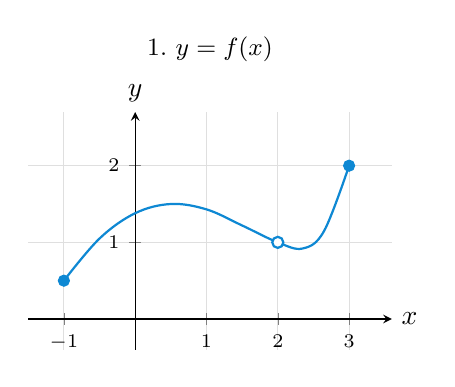
\begin{tikzpicture}
\begin{axis}[grafik, width=6.2cm, height=4.6cm, clip=false, xmin=-1.5, xmax=3.6, ymin=-0.4, ymax=2.7,
  xtick={-1,...,3}, ytick={1,2}, title={\small 1.\ $y = f(x)$}]
  \addplot[thick, cyan!70!blue, smooth, tension=0.6] coordinates
    {(-1,0.5) (-0.5,1.05) (0,1.38) (0.5,1.5) (1,1.43) (1.5,1.22) (2,1) (2.35,0.92) (2.65,1.15) (3,2)};
  \filldraw[cyan!70!blue] (axis cs:-1,0.5) circle (2pt);
  \filldraw[cyan!70!blue, fill=white, thick] (axis cs:2,1) circle (2pt);
  \filldraw[cyan!70!blue] (axis cs:3,2) circle (2pt);
\end{axis}
\end{tikzpicture}
&
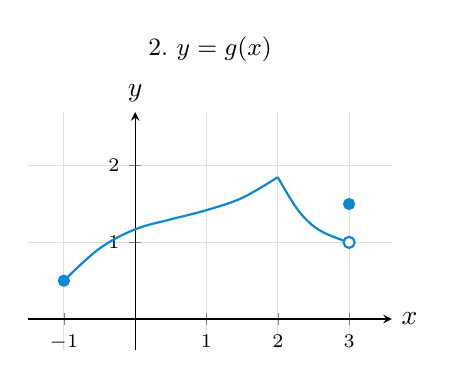
\begin{tikzpicture}
\begin{axis}[grafik, width=6.2cm, height=4.6cm, clip=false, xmin=-1.5, xmax=3.6, ymin=-0.4, ymax=2.7,
  xtick={-1,...,3}, ytick={1,2}, title={\small 2.\ $y = g(x)$}]
  \addplot[thick, cyan!70!blue, smooth, tension=0.6] coordinates
    {(-1,0.5) (-0.5,0.92) (0,1.17) (0.5,1.3) (1,1.42) (1.5,1.58) (2,1.85)};
  \addplot[thick, cyan!70!blue, smooth, tension=0.6] coordinates
    {(2,1.85) (2.3,1.4) (2.6,1.15) (3,1)};
  \filldraw[cyan!70!blue] (axis cs:-1,0.5) circle (2pt);
  \filldraw[cyan!70!blue, fill=white, thick] (axis cs:3,1) circle (2pt);
  \filldraw[cyan!70!blue] (axis cs:3,1.5) circle (2pt);
\end{axis}
\end{tikzpicture}
\\[2ex]
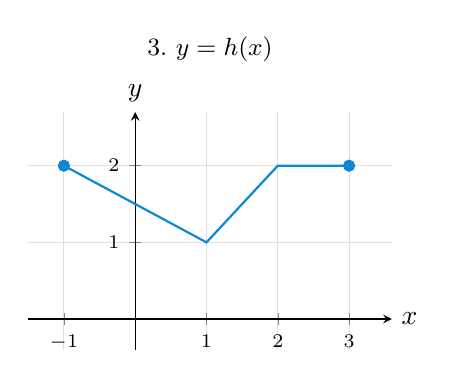
\begin{tikzpicture}
\begin{axis}[grafik, width=6.2cm, height=4.6cm, clip=false, xmin=-1.5, xmax=3.6, ymin=-0.4, ymax=2.7,
  xtick={-1,...,3}, ytick={1,2}, title={\small 3.\ $y = h(x)$}]
  \addplot[thick, cyan!70!blue, no marks] coordinates {(-1,2) (1,1) (2,2) (3,2)};
  \filldraw[cyan!70!blue] (axis cs:-1,2) circle (2pt);
  \filldraw[cyan!70!blue] (axis cs:3,2) circle (2pt);
\end{axis}
\end{tikzpicture}
&
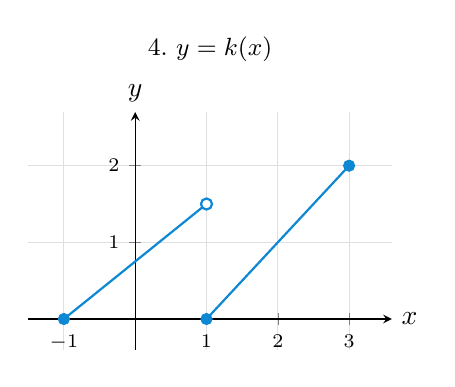
\begin{tikzpicture}
\begin{axis}[grafik, width=6.2cm, height=4.6cm, clip=false, xmin=-1.5, xmax=3.6, ymin=-0.4, ymax=2.7,
  xtick={-1,...,3}, ytick={1,2}, title={\small 4.\ $y = k(x)$}]
  \addplot[thick, cyan!70!blue, no marks] coordinates {(-1,0) (1,1.5)};
  \addplot[thick, cyan!70!blue, no marks] coordinates {(1,0) (3,2)};
  \filldraw[cyan!70!blue] (axis cs:-1,0) circle (2pt);
  \filldraw[cyan!70!blue, fill=white, thick] (axis cs:1,1.5) circle (2pt);
  \filldraw[cyan!70!blue] (axis cs:1,0) circle (2pt);
  \filldraw[cyan!70!blue] (axis cs:3,2) circle (2pt);
\end{axis}
\end{tikzpicture}
\end{tabular}
\end{center}

Untuk setiap grafik fungsi di atas, tentukan di titik mana saja fungsi tersebut kontinu kiri, kontinu kanan, atau tidak kontinu.

\textbf{Jawab:}
\begin{itemize}
\item \textbf{Langkah 1: Tentukan Titik yang Perlu Diperiksa}

Keempat fungsi terdefinisi pada selang $[-1, 3]$. Titik yang perlu diperiksa adalah ujung selang ($x = -1$ dan $x = 3$) serta titik tempat grafik berlubang, melompat, atau berganti aturan.
Di ujung kiri $x = -1$ fungsi hanya dapat didekati dari kanan, dan di ujung kanan $x = 3$ hanya dari kiri.
Nilai fungsi dibaca dari titik penuh ($\bullet$); titik kosong ($\circ$) bukan nilai fungsi.

\item \textbf{Langkah 2: Grafik 1, $y = f(x)$}

\begin{itemize}
  \item $x = -1$: $f(-1) = 0{,}5$ dan kurva di kanannya berawal di titik ini, jadi \textbf{kontinu kanan}.
  \item $x = 2$: hanya ada titik kosong $(2,1)$, sehingga $f(2)$ tidak ada (syarat ke-1 gagal). Walaupun $\lim_{x \to 2} f(x) = 1$ ada, $f$ \textbf{tidak kontinu} di $x = 2$, dan bukan kontinu kiri maupun kontinu kanan.
  \item $x = 3$: $f(3) = 2 = \lim_{x \to 3^-} f(x)$, jadi \textbf{kontinu kiri}.
\end{itemize}
Di titik lain pada $(-1, 3)$ kurva tersambung, sehingga $f$ kontinu. Diskontinuitas di $x = 2$ dapat dihilangkan dengan mendefinisikan $f(2) = 1$.

\item \textbf{Langkah 3: Grafik 2, $y = g(x)$}

\begin{itemize}
  \item $x = -1$: $g(-1) = 0{,}5$ dan kurva berawal di titik ini, jadi \textbf{kontinu kanan}.
  \item $x = 2$: grafik membentuk sudut lancip, tetapi tidak terputus; limit kiri dan kanan sama dengan $g(2)$, jadi $g$ \textbf{kontinu} di $x = 2$ (sekaligus kontinu kiri dan kanan).
  \item $x = 3$: titik penuh $(3, 1{,}5)$ memberi $g(3) = 1{,}5$, sedangkan kurva dari kiri menuju titik kosong $(3,1)$, sehingga
  \[
  \lim_{x \to 3^-} g(x) = 1 \neq 1{,}5 = g(3).
  \]
  Jadi $g$ \textbf{tidak kontinu kiri} di $x = 3$. Karena $x = 3$ ujung kanan selang, $g$ \textbf{tidak kontinu} di $x = 3$.
\end{itemize}
Di titik lain pada $(-1, 3)$, $g$ kontinu.

\item \textbf{Langkah 4: Grafik 3, $y = h(x)$}

\begin{itemize}
  \item $x = -1$: $h(-1) = 2$ dan kurva berawal di titik ini, jadi \textbf{kontinu kanan}.
  \item $x = 1$ dan $x = 2$: grafik berbelok, tetapi tersambung, jadi $h$ \textbf{kontinu} di kedua titik.
  \item $x = 3$: $h(3) = 2 = \lim_{x \to 3^-} h(x)$, jadi \textbf{kontinu kiri}.
\end{itemize}
Tidak ada lubang maupun lompatan, sehingga $h$ kontinu pada seluruh selang tertutup $[-1, 3]$.

\item \textbf{Langkah 5: Grafik 4, $y = k(x)$}

\begin{itemize}
  \item $x = -1$: $k(-1) = 0$ dan kurva berawal di titik ini, jadi \textbf{kontinu kanan}.
  \item $x = 1$: titik penuh $(1,0)$ memberi $k(1) = 0$. Dari kanan, kurva berawal di $(1,0)$; dari kiri, kurva menuju titik kosong $(1, 1{,}5)$:
  \[
  \lim_{x \to 1^-} k(x) = 1{,}5 \neq 0 = k(1), \qquad \lim_{x \to 1^+} k(x) = 0 = k(1).
  \]
  Jadi $k$ \textbf{kontinu kanan} di $x = 1$, tetapi tidak kontinu kiri, sehingga $k$ \textbf{tidak kontinu} di $x = 1$ (diskontinuitas lompat).
  \item $x = 3$: $k(3) = 2 = \lim_{x \to 3^-} k(x)$, jadi \textbf{kontinu kiri}.
\end{itemize}

\item \textbf{Langkah 6: Ringkasan}

\begin{center}
\begin{tabular}{c|c|c|c}
Grafik & Kontinu kiri & Kontinu kanan & Tidak kontinu \\ \hline
$f$ & $x = 3$ & $x = -1$ & $x = 2$ \\
$g$ & -- & $x = -1$ & $x = 3$ \\
$h$ & $x = 3$ & $x = -1$ & -- \\
$k$ & $x = 3$ & $x = -1$ dan $x = 1$ & $x = 1$
\end{tabular}
\end{center}
Di titik selain yang tercantum, setiap fungsi kontinu (sekaligus kontinu kiri dan kontinu kanan).
% final: f: \text{kontinu kanan di } x = -1, \text{ kontinu kiri di } x = 3, \text{ tidak kontinu di } x = 2
% final: g: \text{kontinu kanan di } x = -1, \text{ tidak kontinu di } x = 3
% final: h: \text{kontinu kanan di } x = -1, \text{ kontinu kiri di } x = 3
% final: k: \text{kontinu kanan di } x = -1 \text{ dan } x = 1, \text{ kontinu kiri di } x = 3, \text{ tidak kontinu di } x = 1
\end{itemize}

\end{enumerate}

\end{document}
